\chapter{Communication in the Swarm}

\paragraph*{}
Communication in the Swarm has been mostly wrapped up, with unexpected scenarios accounted for, such as communication failures and conflicts in claiming to be the \textit{"taskmaster"}, the state in which a swarm member claims to be the master of the collective movement and takes on the responsibility of conducting path planning. However, the integration with the actual flow still remains, which is our next step with regards to the communication. Our prerequisite for this integration will be when multiple robots are able to move autonomously, which is our next milestone.

\paragraph*{}
With the transition from the simulation to an actual physical implementation, we have decided to proceed with using socket communication as the core method. In addition, to handle unexpected failures, retry functionalities have been implemented by following an architecture similar to the "Three way handshake" of the Transmission Control Protocol, by checking for acknowledgements and retry if there are no acknowledgements from the intended receivers.

\paragraph*{}
Another key highlight for the communication will be how it handles conflicting taskmaster claims. A taskmaster claim will occur by the swarm member has detected an object. In the instance that more than one swarm robot claims to be the taskmaster at once, the swarm will refer to a priority queue and resolves the conflicting claims by appointing the claim by the member higher on the priority queue as the taskmaster. After that, they will reconfirm with the swarm to ensure that the taskmaster is matching.

\paragraph*{}
After the taskmaster has been appointed, the current positions of all the swarm members will be transmitted to the taskmaster for path planning. This position will be obtained while the robot is stationary since once an object is detected, a broadcast is sent to stop any ongoing movements of all the robots in the swarm. Thus, our path planning algorithm can be invoked. The flow for communication is attached below. (Figure \ref{fig:communication-flow})

\begin{figure}[H]
    \centering
    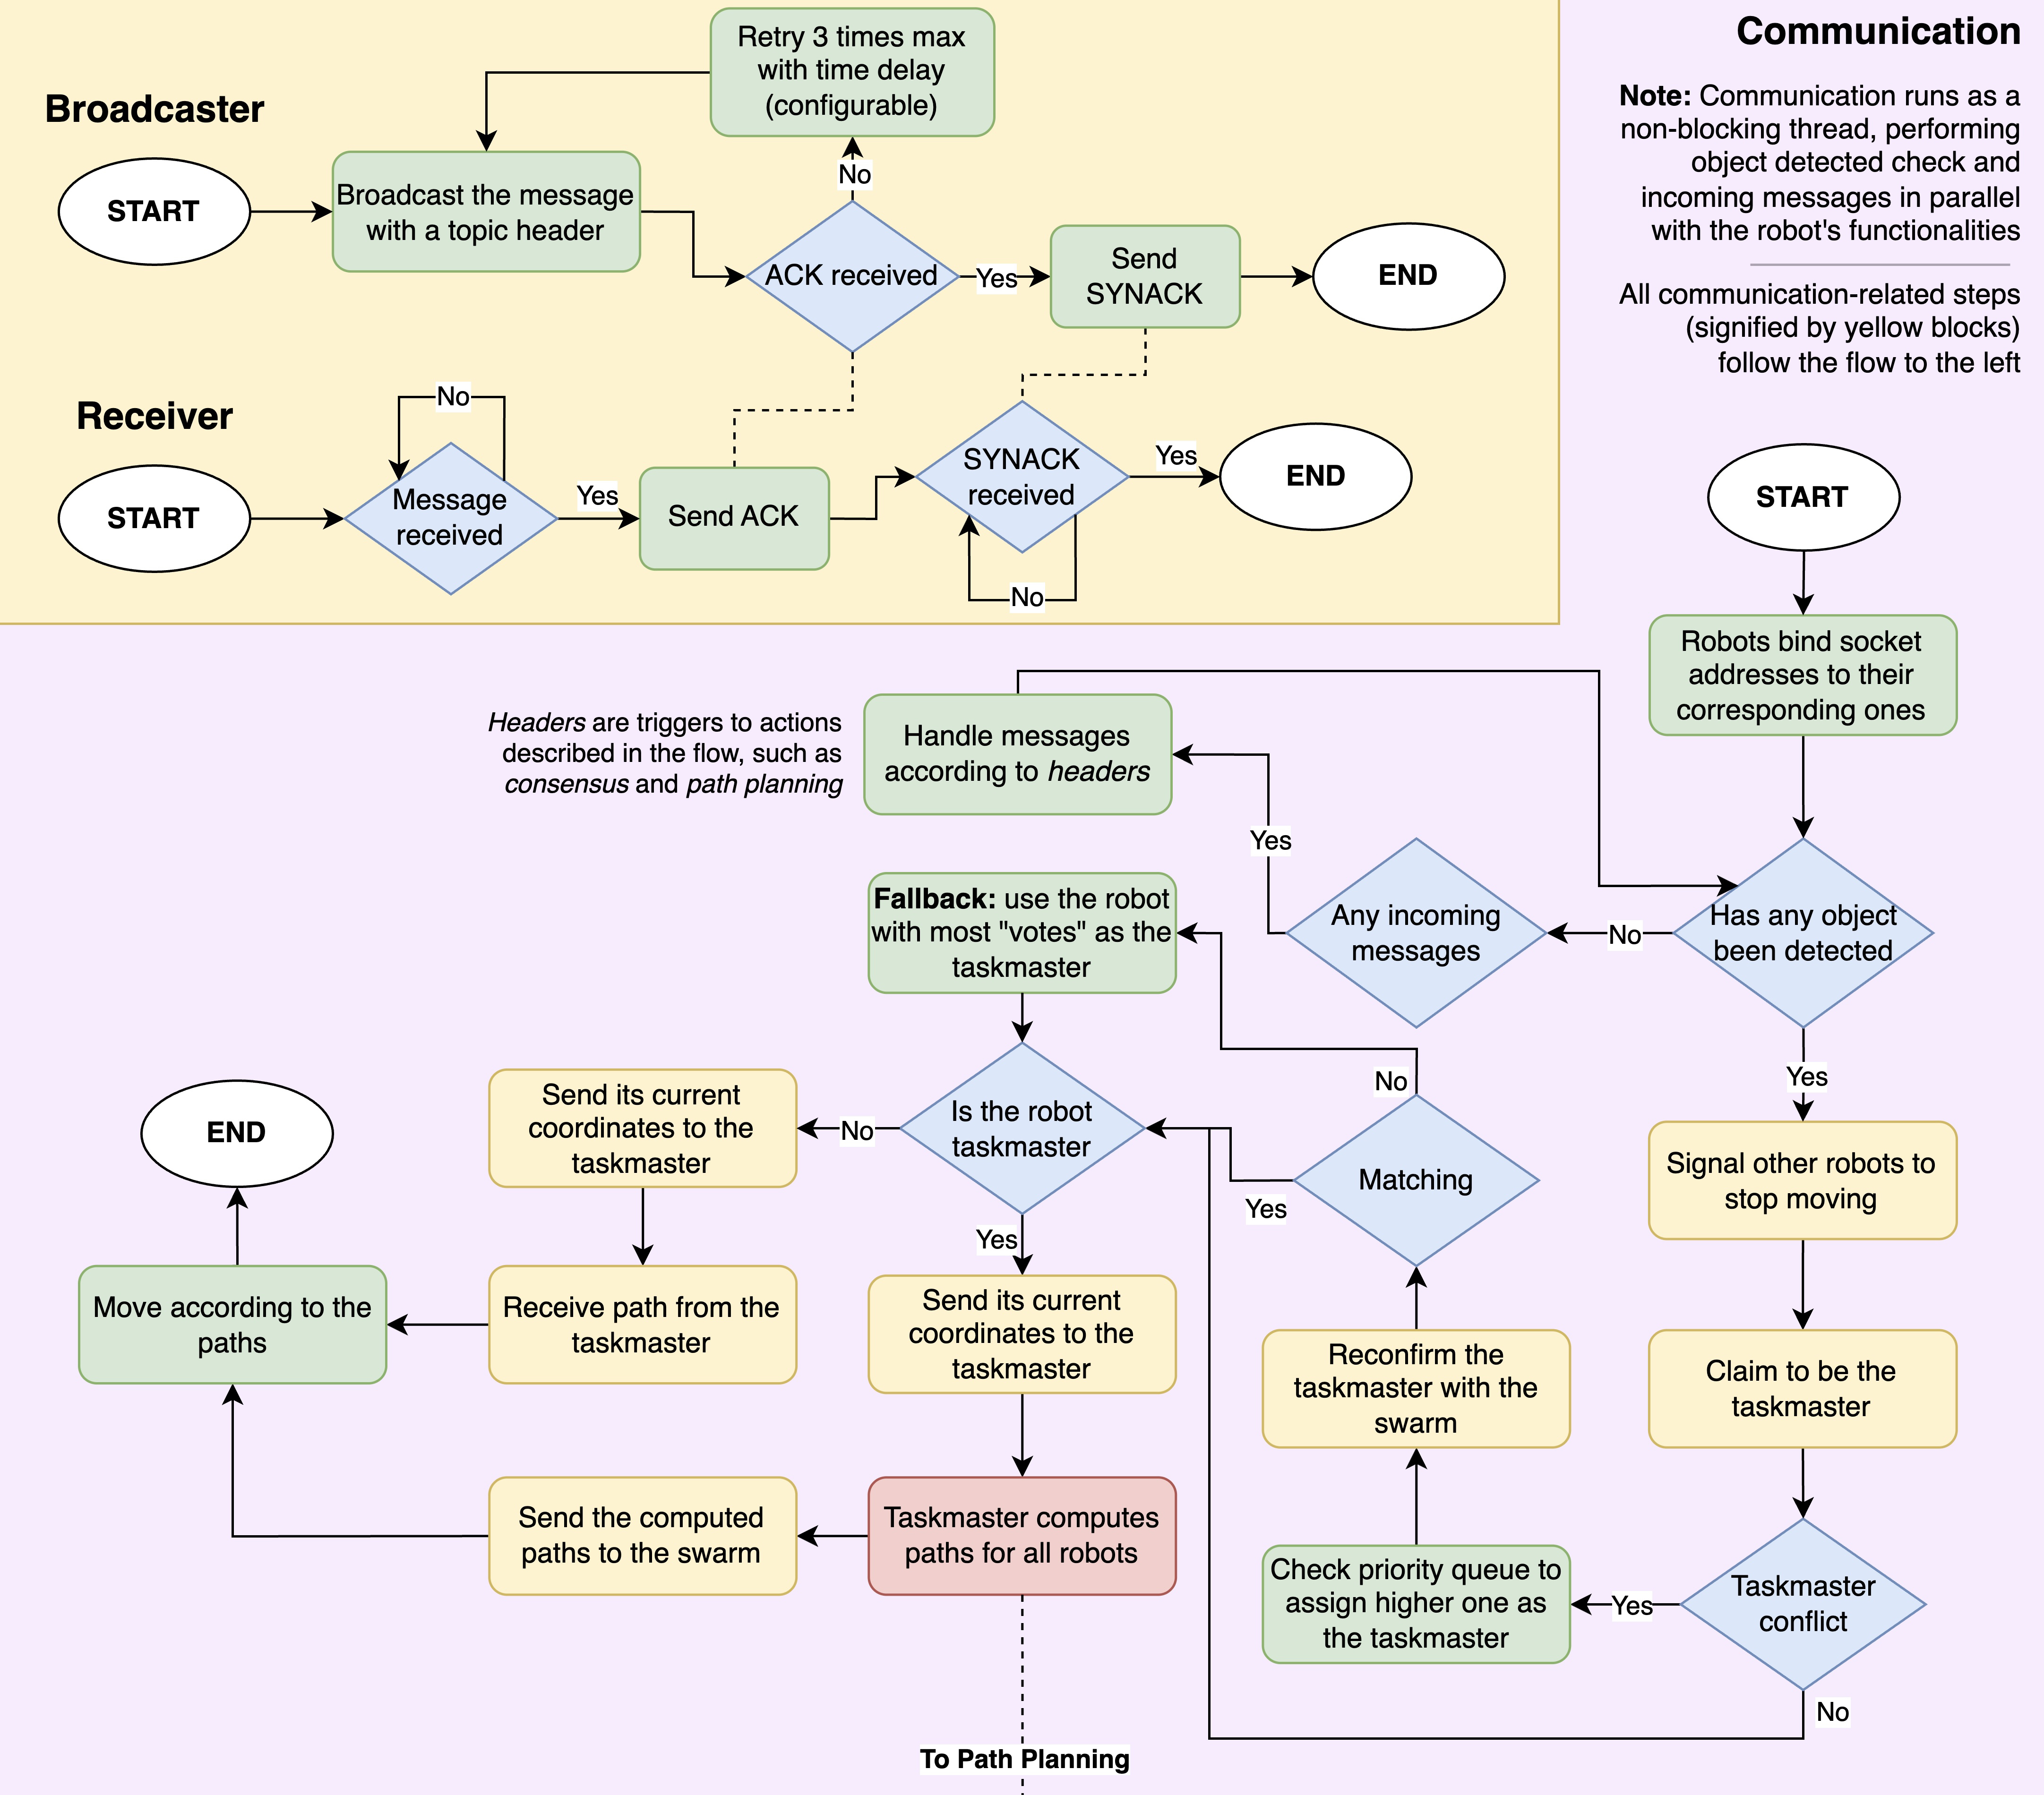
\includegraphics[width=0.9\linewidth]{assets/images/communication/communication-flow.png}
    \caption{Communication in the Swarm Detailed Flow}
    \label{fig:communication-flow}
\end{figure}
